Die Parametrisierung der beiden Templates erfolgt durch die sogenannte $\chi^{2}$-Minimierung.
$\chi^{2}$ gibt dabei als ein Maß an, wie gut eine Verteilung an gegebene Daten passt.
Je kleiner $\chi^{2}$ ist, umso besser beschreibt die Verteilung die Daten, deshalb wird $\chi^{2}$ bei der Parametrisierung minimiert.
Als freie Parameter werden zwei Skalierungsfaktoren benutzt, einmal ein Skalierungsfaktor für das Template des Signals (SF\textsubscript{Signal}) und einmal ein Skalierungsfaktor für das Template des korrelierten Untergrunds (SF\textsubscript{korr. Untergrund}).
Für $\chi^{2}$ gilt dann:
\begin{align}
\chi^{2} = \sum_{i}\left(\frac{\text{SF}_\text{Signal}\cdot x_{i}+\text{SF}_\text{korr. Untergrund}\cdot y_{i}-z_{i}}{\sqrt{\left(\text{SF}_\text{Signal}\cdot\Delta x_{i}\right)^{2}+\left(\text{SF}_\text{korr. Untergrund}\cdot\Delta y_{i}\right)^{2}+\left(\Delta z\right)^{2}}}\right)^{2}
\label{eq:Chi2}
\end{align}
Hierbei steht $x$ für das Template des Signals, $y$ für das Template des korrelierten Untergrunds und $z$ für die Verteilung der invarianten Masse nach Abzug der unkorrelierten Untergrunds.
Der Index $i$  symbolisiert, dass über die verschiedenen Werte der invarianten Masse summiert wird.
\begin{figure}[tp]
\centering
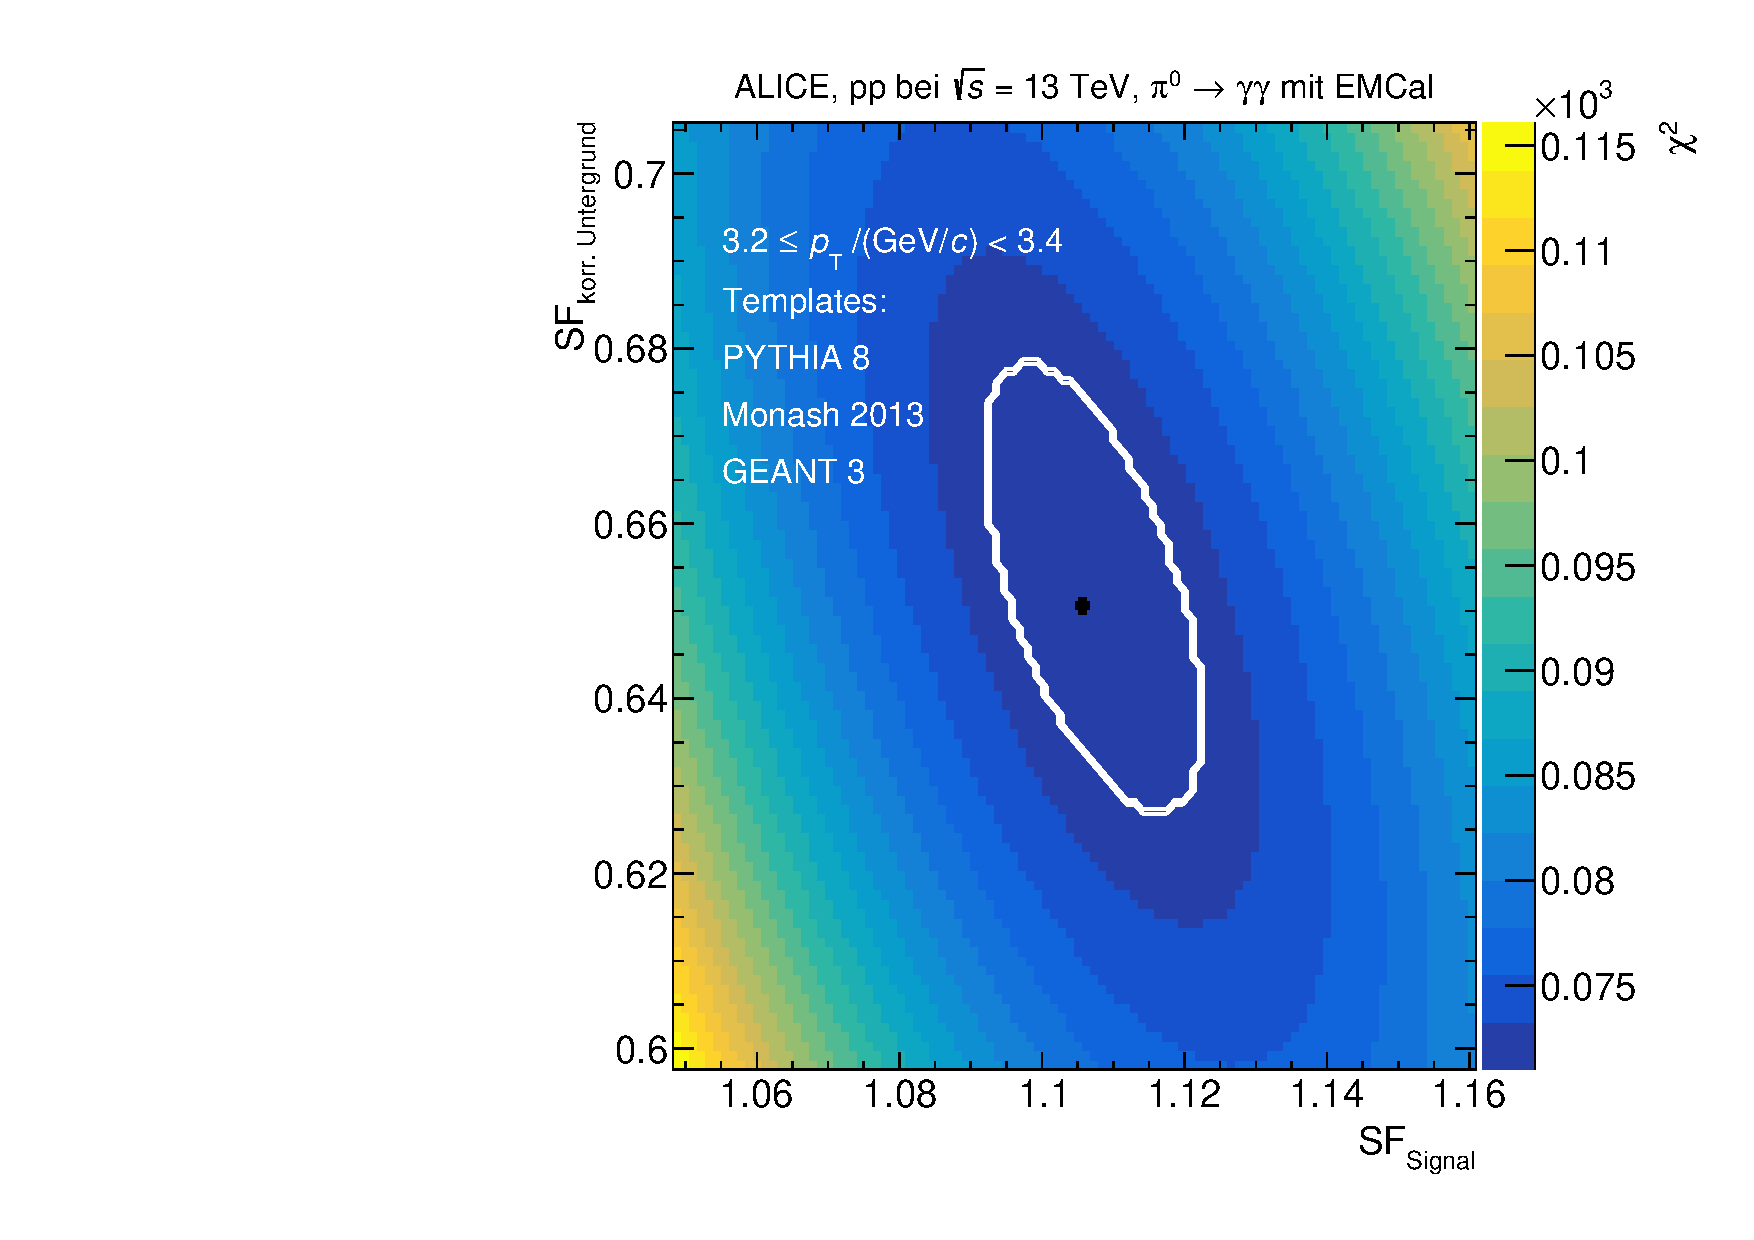
\includegraphics[width=.65\linewidth]{Chi2Map10_Data_2016.pdf}
\caption{$\chi^{2}$ in Abhängigkeit der Skalierungsfaktoren für das Template des Signals und das Template des korrelierten Untergrunds in einem $p_{\text{T}}$-Intervall von $(3\,2 - 3\,4)(\text{GeV}/c)$.
Die weiße Kurve makiert die Unsicherheit auf $\chi^{2}_\text{min}$.}
\label{fig:Chi2Map}
\end{figure}
\newline
Abbildung \ref{fig:Chi2Map} zeigt eine Verteilung von $\chi^{2}$ für unterschiedliche Kombinationen der beiden Skalierungsfaktoren in einem $p_{\text{T}}$-Intervall von $(3\,2 - 3\,4)(\text{GeV}/c)$.
Die weiße Kurve umrahmt das Minimum $\chi^{2}_\text{min}$ und gibt die Unsicherheit bezüglich der beiden Skalierungsfaktoren an.
Die Werte die auf der weißen Kurve liegen bei $\chi^{2}_\text{min}+1$ \cite{book:chi2}.
